\section{Metoda emitowania światła strukturalnego}
Skanery oparte o metodę emitowania światła strukturalnego wyświetlają siatkę świetlną na mierzony obiekt. Następnie wzór na obiekcie jest mierzony przez jedną lub dwie kamery. Za sprawą badania mocy światła odbitego oraz kształtu siatki na przedmiocie, korzystając z metod triangulacji, można wyznaczyć położenie obiektu w innym układzie współrzędnych. Jednocześnie wskutek wykorzystania obrazu z dwóch kamer jest możliwe wykonanie pełnego zdjęcia 3D. Głównym walorem tej metody jest możliwość wykonywania zdjęć z dużą częstotliwością. Ponadto światło emitowane przez ten skaner nie jest światłem laserowym, dlatego też wszelkie aspekty zagrażające wzrokowi są wyeliminowane \cite{nowacki2018pomiar}. Słabym punktem tej metody jest ograniczona gęstość rzutowanej siatki. Co w przypadku obiektu o skomplikowanym kształcie sprawia,iż pomiar będzie musiał być wykonany parokrotnie pod różnymi kątami w celu uzyskania dokładnych wyników \cite{nowacki2018pomiar}. Zasada działania skanera bazującego na metodzie emitowania światła strukturalnego została przedstawiona na rysunku ~\ref{fig:structureLightPic1}.

\begin{figure}[H]
  \centering
  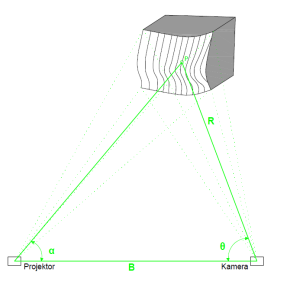
\includegraphics[scale=0.75]{swiatlostrukturalne.PNG}
  \caption{Metoda wyznaczania współrzędnych w technice światła strukturalnego \cite{Wrona_Piotrowska_2015}.}   
  \label{fig:structureLightPic1}
\end{figure}
\newline
Korzystając z podstawowych zależności trygonometrycznych możliwe jest wyprowadzenie równań pozwalających na wyznaczenie odległości poszczególnych punktów mierzonego obiektu od kamery.
\begin{equation}
    \begin{aligned}
        & \frac{R}{sin(\alpha)}=\frac{B}{sin(180-\alpha-\theta)} \\
          & R=B\frac{sin(\theta)}{sin(\alpha+\theta)} \\
    \end{aligned}
\end{equation}
$\alpha$ to kąt pomiędzy wiązką światła emitowanego przez projektor, a odcinkiem łączącym projektor oraz kamerę. $\theta$ jest kątem pomiędzy wiązką światła docierającą do kamery, a odcinkiem łączącym projektor oraz kamerę. B to odległość pomiędzy kamerą, a projektorem. R jest odległością kamery od mierzonego przedmiotu.

W tabeli ~\ref{tab:faroscanboxTab} zostały przedstawione charakterystyki urządzenia Faro Scan in a box.
\begin{table}[H]
\begin{center}

\caption{\label{tab:faroscanboxTab}Charakterystyki skanera Faro Scan in a box \cite{siabDatasheet}.}
\centerline{
\begin{tabular}{ |c| c| }
 \hline
 {\small Zasięg} & {\small 0.2 m-1.12 m}\\ 
  \hline
 {\small Gęstość siatki} & {\small 0.078 mm-0.39 mm}\\  
 \hline
 {\small Prędkość pomiaru} & {\small $<4$ s} \\  
  \hline
 {\small Gęstość meshu} & {\small Do 10 mln wierzchołków}  \\  
  \hline
   {\small Dokładność } & {\small Do  0.1 \% wielkości obiektu} \\  
  \hline

\end{tabular}
}

\end{center}
\end{table}
Ze względu na krótki zasięg pomiaru skanery korzystające z metody emitowania światła strukturalnego nadają się jedynie do pomiarów krótkodystansowych. Ten sposób pomiarowy jest wykorzystywany w urządzeniach takich jak Xbox Kinnect oraz kamerach RGBD firmy Intel. Gęstość siatki generowanej na obiekcie mierzonym jest bardzo duża, przez co dokładność odwzorowania takich modeli znacznie przewyższa inne metody pomiarów 3D. Ponadto przy wykonywaniu pomiaru, dokonywany jest skan całej powierzchni obiektu na którą trafiło emitowane światło. Wpływa to znacznie na prędkość pomiaru, ponieważ przy jednej obserwacji jest możliwe uchwycenie nawet połowy obiektu, o ile cały został umieszczony w kadrze kamery.